\documentclass[11pt]{standalone}
\usepackage{tikz, pgfplots,amsmath, amssymb, amsthm}   
\usepgfplotslibrary{groupplots}


\begin{document}


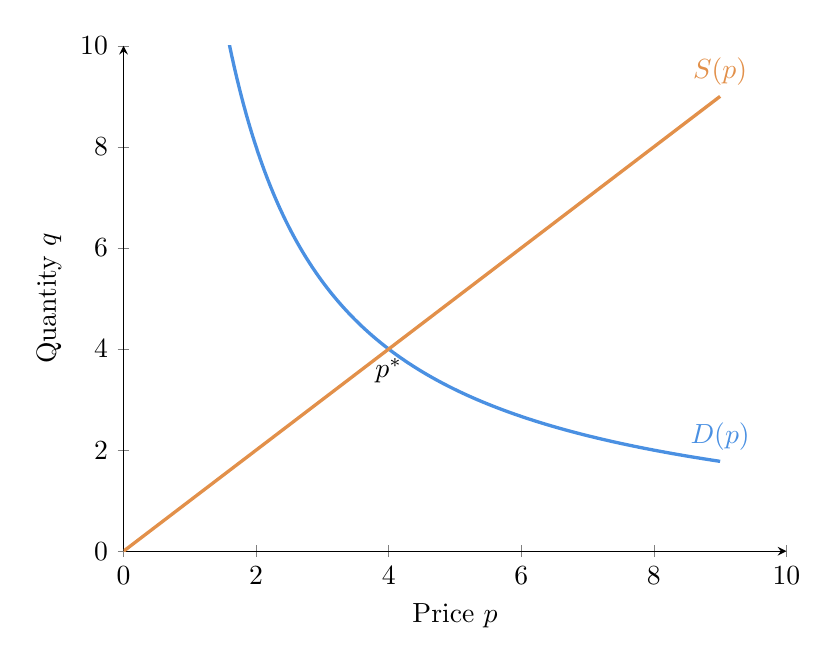
\begin{tikzpicture}[scale=1]
\begin{axis}[
  	height=8cm, width=10cm,
	axis x line=bottom, axis y line=left,
   	xlabel = Price $p$, ylabel = Quantity $q$,
  	ymin=0, ymax=10, xmin=0, xmax=10,
]
    
\addplot[black]  coordinates {(4, 4)} node[anchor=north] {$p^*$};
\addplot[color={rgb, 255:red, 74; green, 144; blue, 226 }, very thick,  domain=0:9, samples=200, variable=\t]({t},  {16/t)} )node[above] {$D(p)$} ;
\addplot[color={rgb, 255:red, 226; green, 144; blue, 74 }, very thick,  domain=0:9, samples=1000, variable=\t]({t},  {t)} )node[above] {$S(p)$} ;
\end{axis}
\end{tikzpicture}



\end{document}